\documentclass[CheckpointReport.tex]{subfiles}
\begin{document}

\bigskip

\section*{\textsc{\Large Progress}}
Various locks, including the CLH lock, MCS Lock, Bakery Lock, and Szyma\`{n}ski's Algorithm have been implemented.  Using these algorithms, tests are being done to compare execution times.  The Szyma\`{n}ski's Algorithm is still having some data race bugs and thread failure bugs, therefore it is not included in these tests.  We also use the Java Reentrant Lock as a good base point for our testing and comparison to our own locks.  

One of the tests we have performed already is that of simple counting.  The threads will concurrently increment a counter variable, which is shared between all the threads, and using one of the aforementioned locks.

\begin{figure}[H]
	\centering
	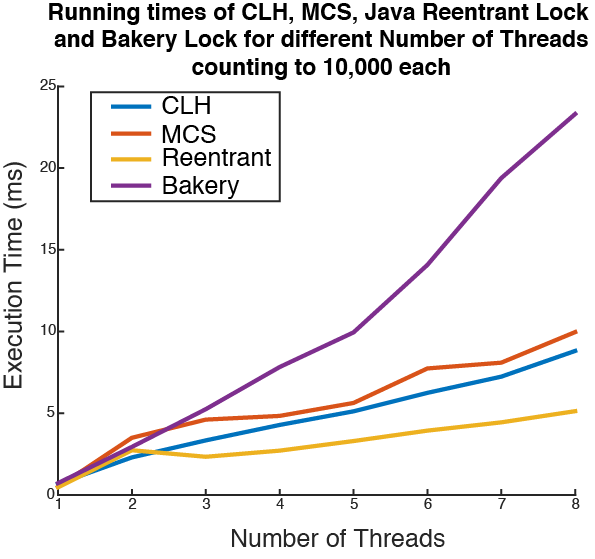
\includegraphics[]{runningTime.png}
\end{figure}
\end{document}